% this file is called up by thesis.tex
% content in this file will be fed into the main document

%: ----------------------- name of chapter  -------------------------
\appendix
\chapter{Appendix} % top level followed by section, subsection

\section{Repositories}\label{appendix:repos}
\begin{table}[H]
\centering
\begin{tabular}{l|l}
\textbf{Repository}                                         & \textbf{Commit hash}                                  \\\hline
\pbox{5cm}{https://github.com/Luc-Veldhuis/MasterThesisCS2020} & d3bdae47ed5a231414bb5b9ef2858d9cbe58a1b1 \\
https://github.com/Luc-Veldhuis/Angora             & 41a75f4c0bc411c37c310fa1f4e71be71212af67 \\
https://github.com/Luc-Veldhuis/symcc              & 363a3deb5064f03d2f6b558e6082961c9f46ce73 \\
https://github.com/file/file                       & 87731415de945660b00f02207d8e9d986ef9b82e \\
https://github.com/oelbrenner/jhead                & 9c34b3b8c1cda921c6f629866a956bd1ac8dbc11 \\
https://github.com/libexpat/libexpat               & a7bc26b69768f7fb24f0c7976fae24b157b85b13 \\
https://github.com/LuaDist/libjpeg                 & 6c0fcb8ddee365e7abc4d332662b06900612e923 \\
git://sourceware.org/git/binutils-gdb.git          & b5624945ea67525c0ba4ffec7a9d3f9366bf9071 \\
https://github.com/madler/zlib                                               &           cacf7f1d4e3d44d871b605da3b647f07d718623f                               \\
https://github.com/glennrp/libpng                                             &          a40189cf881e9f0db80511c382292a5604c3c3d1                                \\
https://gitlab.com/esr/gif2png                                            &             d9c6b36c2dbcfee2a7cafe2ee5b3848b4631167c                            
\end{tabular}
\caption{Source of used repositories and their commit hashes.}
\label{table:repoversions}
\end{table}

\section{Comparing metrics per program}
In Figure \ref{fig:kde-flipped-conditions}, we see the kernel density estimation of every metric when considering only the flipped conditions per program. A high resolution image can be found at \footnote{\url{https://github.com/Luc-Veldhuis/MasterThesisCS2020/tree/0.2/analysis/graphs/kde_flipped_conditions.png}}.
\begin{figure}[p]
    \centering
    % include first image
    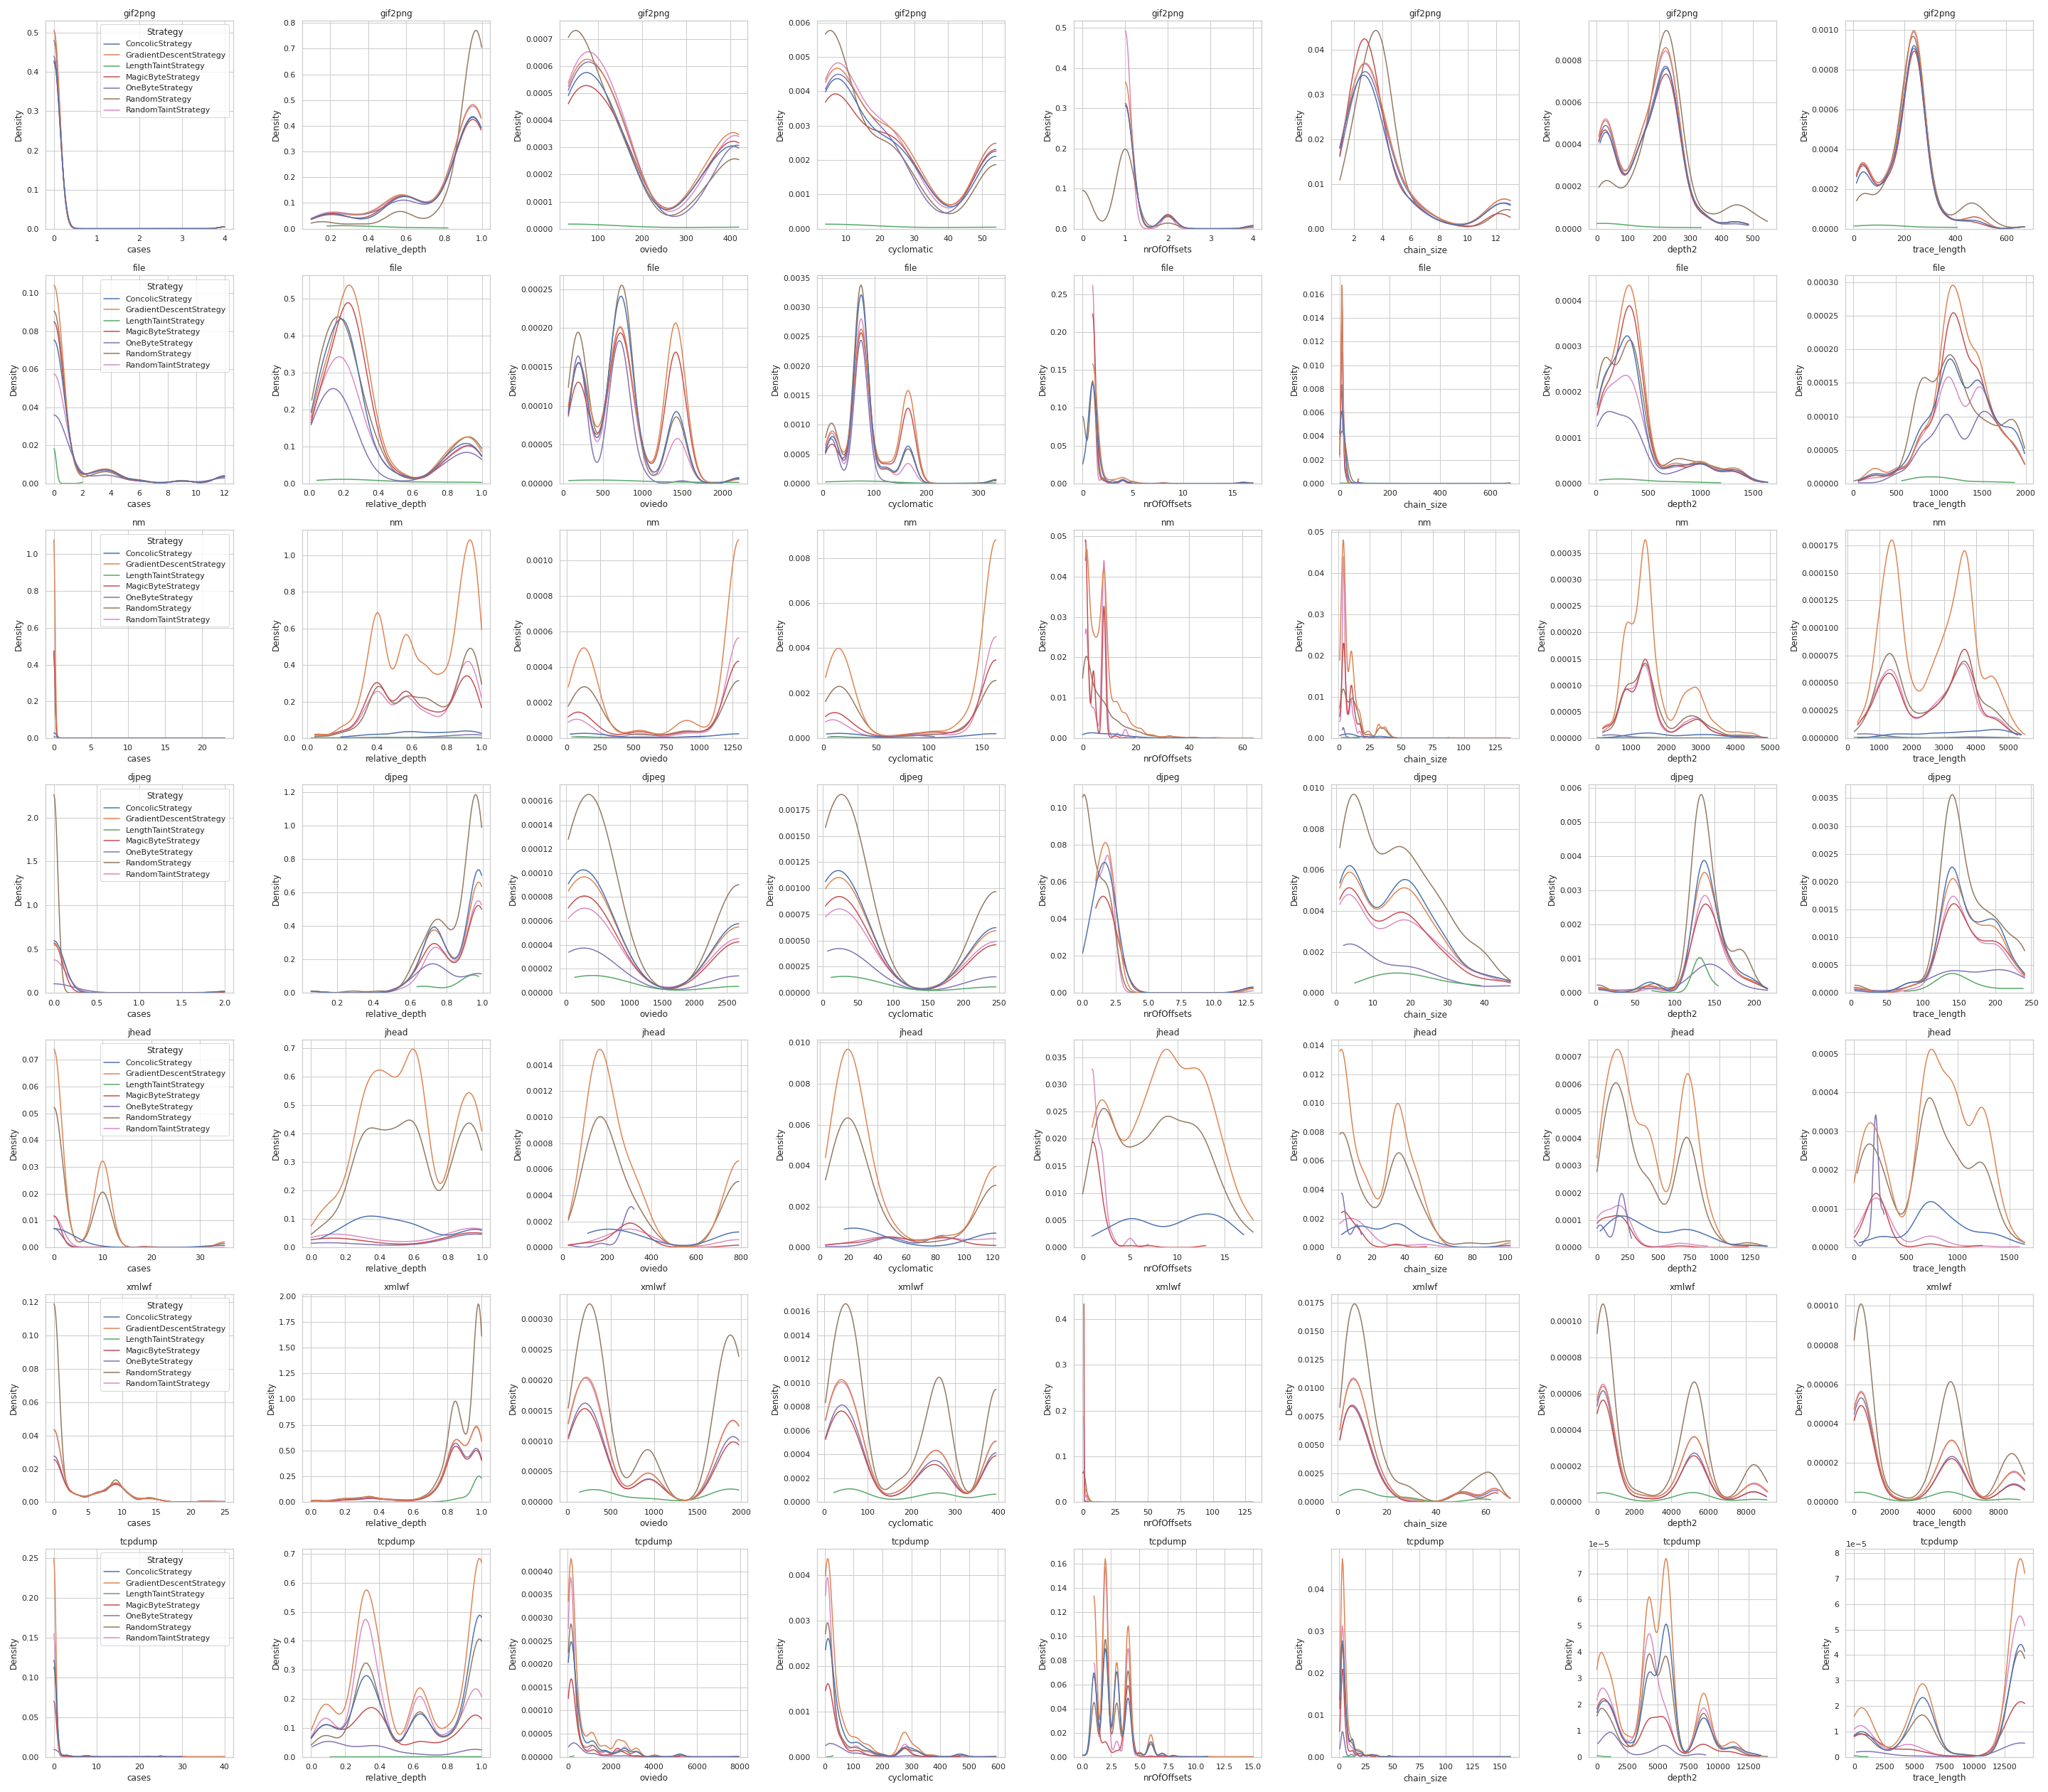
\includegraphics[width=\textheight,height=\textwidth,keepaspectratio, angle=90]{5_results/graphs_new/kde_flipped_conditions.png}  
    \caption{Kernel density estimation plots of metrics per program}
    \label{fig:kde-flipped-conditions}
\end{figure}

\section{Machine learning models}\label{appendix:models}
In Table \ref{tab:classifiers-overview}, we show the classifier models and the hyper parameters which are searched. The parameters correspond to the models in the scikit-learn library \cite{scikit-learn}. All data is first standardized using the RobustScaler.
\begin{table}[H]
\centering
\begin{tabular}{ll}
\toprule
        Model &                                                                                Parameters \\
\midrule
    LinearSVC &                                                          $C\in \{1, 10, 100, 1000, 10000\}$ \\
          SVC &                     $C\in \{1, 10, 100, 1000, 10000\}$\\ & $gamma\in \{0.001, 0.01, 0.1, scale\}$ \\
        NuSVC &                                                      $gamma\in \{0.001, 0.01, 0.1, scale\}$ \\
      Gausian &                                                            $multi\_class\in \{one\_vs\_rest\}$ \\
 DecisionTree &  $min\_samples\_leaf\in \{1, 2, 4, 8, 16\}$\\ & $max\_depth\in \{None, 256, 512, 1024, 2048, 4096\}$ \\
\bottomrule
\end{tabular}

\caption{Classifiers tried and their search-space.}\label{tab:classifiers-overview}
\end{table}

In Table \ref{tab:regressor-overview}, we show the regression models and the hyper parameters which are searched. Again the parameters correspond to the model parameters from the scikit-learn library \cite{scikit-learn}. All data is first standardized using the RobustScaler.
\begin{table}[H]
\centering
\begin{tabular}{ll}
\toprule
                    Model &                                                                               Parameters \\
\midrule
         LinearRegression &                                                                   $normalize\in \{False\}$ \\
                    Ridge &                                                 $alpha\in \{0.01, 0.1, 1, 10, 100, 1000\}$ \\
               ElasticNet &                                                 $alpha\in \{0.01, 0.1, 1, 10, 100, 1000\}$ \\
                    Lasso &                                                 $alpha\in \{0.01, 0.1, 1, 10, 100, 1000\}$ \\
           MultiTaskLasso &                                                 $alpha\in \{0.01, 0.1, 1, 10, 100, 1000\}$ \\
                      SVR &                     $C\in \{1, 10, 100, 1000, 10000\}$\\ & $gamma\in \{0.001, 0.01, 0.1, scale\}$ \\
                    NuSVR &                                                     $gamma\in \{0.001, 0.01, 0.1, scale\}$ \\
                LinearSVR &                                                         $C\in \{1, 10, 100, 1000, 10000\}$ \\
             SGDRegressor &                                                    $alpha\in \{0.0001, 0.001, 0.01, 0.1\}$ \\
 GaussianProcessRegressor &                                    $alpha\in \{10^{-10}, 10^{-9}, 10^{-8}, 10^{-7}, 10^{-6}, 10^{-5}\}$ \\
    DecisionTreeRegressor &  $min\_samples\_leaf\in \{1, 2, 4, 8, 16\}$\\ & $max\_depth\in \{None, 256, 512, 1024, 2048, 4096\}$ \\
\bottomrule
\end{tabular}

\caption{Regressors tried and their search-space}\label{tab:regressor-overview}
\end{table}

%: ----------------------- paths to graphics ------------------------

% change according to folder and file names

%: ----------------------- contents from here ------------------------
\begin{comment}
\section{Gradient Descent Algorithm}\label{appendix:gdAlgo}
\todo{Explain get\_output function}.
\begin{figure}[H]
    \centering
    \lstinputlisting[language=Python,breaklines=true]{code/gd.py}
    \caption{High level overview of the Gradient Descent Algorithm}
    \label{fig:gdAlgo}
\end{figure}



\section{Depth totals}\label{appendix:depth}
\begin{table}[H]
\centering
\begin{tabular}{|l|l|}
\hline
\textbf{Depth} & \textbf{Total} \\ \hline
0-9\%             & 14             \\ \hline
10-19\%           & 0              \\ \hline
20-29\%           & 6              \\ \hline
30-39\%           & 11             \\ \hline
40-49\%           & 1              \\ \hline
50-59\%           & 183            \\ \hline
60-69\%           & 218            \\ \hline
70-79\%           & 37             \\ \hline
80-89\%           & 31             \\ \hline
90-100\%          & 10             \\ \hline
\end{tabular}
\caption{Total number of unique conditions per bucket in the \texttt{djpeg} binary}.
\end{table}

\begin{table}[H]
\centering
\begin{tabular}{|l|l|}
\hline
\textbf{Depth} & \textbf{Total} \\\hline
0-9\%             & 1407           \\\hline
10-19\%           & 1051           \\\hline
20-29\%           & 674            \\\hline
30-39\%           & 300            \\\hline
40-49\%           & 267            \\\hline
50-59\%           & 452            \\\hline
60-69\%           & 247            \\\hline
70-79\%           & 177            \\\hline
80-89\%           & 8              \\\hline
90-100\%          & 2              \\ \hline
\end{tabular}
\caption{Total number of unique conditions per bucket in the \texttt{file} binary}.
\end{table}

\begin{table}[H]
\centering
\begin{tabular}{|l|l|}
\hline
\textbf{Depth} & \textbf{Total} \\ \hline
0-9\%             & 117            \\ \hline
10-19\%           & 12             \\ \hline
20-29\%           & 66             \\ \hline
30-39\%           & 112            \\ \hline
40-49\%           & 196            \\ \hline
50-59\%           & 21             \\ \hline
60-69\%           & 20             \\ \hline
70-79\%           & 8              \\ \hline
80-89\%           & 15             \\ \hline
90-100\%          & 4              \\ \hline
\end{tabular}
\caption{Total number of unique conditions per bucket in the \texttt{gif2png} binary}.
\end{table}

\begin{table}[H]
\centering
\begin{tabular}{|l|l|}
\hline
\textbf{Depth} & \textbf{Total} \\ \hline
0-9\%             & 201            \\ \hline
10-19\%           & 272            \\ \hline
20-29\%           & 126            \\ \hline
30-39\%           & 107            \\ \hline
40-49\%           & 83             \\ \hline
50-59\%           & 208            \\ \hline
60-69\%           & 40             \\ \hline
70-79\%           & 2              \\ \hline
80-89\%           & 8              \\ \hline
90-100\%          & 2              \\ \hline
\end{tabular}
\caption{Total number of unique conditions per bucket in the \texttt{jhead} binary}.
\end{table}


\begin{table}[H]
\centering
\begin{tabular}{|l|l|}
\hline
\textbf{Depth} & \textbf{Total} \\ \hline
0-9\%             & 6170           \\ \hline
10-19\%           & 267            \\ \hline
20-29\%           & 262            \\ \hline
30-39\%           & 87             \\ \hline
40-49\%           & 328            \\ \hline
50-59\%           & 2465           \\ \hline
60-69\%           & 506            \\ \hline
70-79\%           & 53             \\ \hline
80-89\%           & 201            \\ \hline
90-100\%          & 775            \\ \hline
\end{tabular}
\caption{Total number of unique conditions per bucket in the \texttt{xmlwf} binary}.
\end{table}


\begin{table}[H]
\centering
\begin{tabular}{|l|l|}
\hline
\textbf{Depth} & \textbf{Total} \\ \hline
0-9\%             & 8998           \\ \hline
10-19\%           & 2809           \\ \hline
20-29\%           & 4240           \\ \hline
30-39\%           & 1350           \\ \hline
40-49\%           & 523            \\ \hline
50-59\%           & 1002           \\ \hline
60-69\%           & 432            \\ \hline
70-79\%           & 371            \\ \hline
80-89\%           & 276            \\ \hline
90-100\%          & 12             \\ \hline
\end{tabular}
\caption{Total number of unique conditions per bucket in the \texttt{nm} binary}.
\end{table}




\section{Offset totals}\label{appendix:offsets}

\begin{table}[H]
\centering
\begin{tabular}{|l|l|}
\hline
\textbf{Offsets} & \textbf{Total} \\ \hline
0                 & 334            \\ \hline
1                 & 79             \\ \hline
2                 & 93             \\ \hline
13                & 5              \\ \hline
\end{tabular}
\caption{Total number of unique conditions per offset in the \texttt{djpeg} binary}.
\end{table}


\begin{table}[H]
\centering
\begin{tabular}{|l|l|}
\hline
\textbf{Offsets} & \textbf{Total} \\ \hline
0                 & 1967           \\ \hline
1                 & 1921           \\ \hline
2                 & 430            \\ \hline
3                 & 145            \\ \hline
4                 & 41             \\ \hline
5                 & 15             \\ \hline
6                 & 4              \\ \hline
8                 & 2              \\ \hline
9                 & 3              \\ \hline
11                & 2              \\ \hline
12                & 1              \\ \hline
14                & 5              \\ \hline
16                & 25             \\ \hline
17                & 11             \\ \hline
30                & 2              \\ \hline
36                & 1              \\ \hline
76                & 2              \\ \hline
89                & 2              \\ \hline
104               & 1              \\ \hline
124               & 1              \\ \hline
126               & 2              \\ \hline
129               & 1              \\ \hline
509               & 1              \\ \hline
\end{tabular}
\caption{Total number of unique conditions per offset in the \texttt{file} binary}.
\end{table}





\begin{table}[H]
\centering
\begin{tabular}{|l|l|}
\hline
\textbf{Offsets} & \textbf{Total} \\ \hline
0                 & 188            \\ \hline
1                 & 333            \\ \hline
2                 & 35             \\ \hline
3                 & 9              \\ \hline
4                 & 5              \\ \hline
14                & 1              \\ \hline
\end{tabular}
\caption{Total number of unique conditions per offset in the \texttt{gif2png} binary}.
\end{table}

\begin{table}[H]
\centering
\begin{tabular}{|l|l|}
\hline
\textbf{Offsets} & \textbf{Total} \\ \hline
0                 & 2              \\ \hline
1                 & 92             \\ \hline
2                 & 126            \\ \hline
3                 & 59             \\ \hline
4                 & 3              \\ \hline
5                 & 63             \\ \hline
6                 & 25             \\ \hline
7                 & 117            \\ \hline
8                 & 32             \\ \hline
9                 & 136            \\ \hline
10                & 2              \\ \hline
11                & 108            \\ \hline
12                & 30             \\ \hline
13                & 145            \\ \hline
14                & 16             \\ \hline
15                & 59             \\ \hline
16                & 6              \\ \hline
17                & 14             \\ \hline
18                & 14             \\ \hline
\end{tabular}
\caption{Total number of unique conditions per offset in the \texttt{jhead} binary}.
\end{table}


\begin{table}[H]
\centering
\begin{tabular}{|l|l|}
\hline
\textbf{Offsets} & \textbf{Total} \\ \hline
0                 & 6136           \\ \hline
1                 & 3931           \\ \hline
2                 & 523            \\ \hline
3                 & 236            \\ \hline
4                 & 63             \\ \hline
5                 & 16             \\ \hline
6                 & 1              \\ \hline
7                 & 38             \\ \hline
8                 & 2              \\ \hline
10                & 4              \\ \hline
11                & 14             \\ \hline
12                & 9              \\ \hline
13                & 1              \\ \hline
14                & 2              \\ \hline
16                & 1              \\ \hline
19                & 1              \\ \hline
44                & 5              \\ \hline
52                & 28             \\ \hline
53                & 12             \\ \hline
56                & 24             \\ \hline
57                & 2              \\ \hline
59                & 5              \\ \hline
61                & 4              \\ \hline
67                & 1              \\ \hline
70                & 2              \\ \hline
71                & 1              \\ \hline
91                & 1              \\ \hline
101               & 1              \\ \hline
109               & 2              \\ \hline
112               & 1              \\ \hline
113               & 8              \\ \hline
116               & 18             \\ \hline
119               & 1              \\ \hline
120               & 5              \\ \hline
121               & 1              \\ \hline
125               & 1              \\ \hline
127               & 8              \\ \hline
131               & 5              \\ \hline
\end{tabular}
\caption{Total number of unique conditions per offset in the \texttt{xmlwf} binary}.
\end{table}


\begin{table}[H]
\centering
\begin{tabular}{|l|l|}
\hline
\textbf{Offsets} & \textbf{Total} \\ \hline
0                 & 1440           \\ \hline
1                 & 4648           \\ \hline
2                 & 2181           \\ \hline
3                 & 1134           \\ \hline
4                 & 1980           \\ \hline
5                 & 728            \\ \hline
6                 & 1218           \\ \hline
7                 & 371            \\ \hline
8                 & 2313           \\ \hline
9                 & 500            \\ \hline
10                & 693            \\ \hline
11                & 309            \\ \hline
12                & 370            \\ \hline
13                & 413            \\ \hline
14                & 395            \\ \hline
15                & 151            \\ \hline
16                & 239            \\ \hline
17                & 176            \\ \hline
18                & 128            \\ \hline
19                & 97             \\ \hline
20                & 103            \\ \hline
21                & 48             \\ \hline
22                & 107            \\ \hline
23                & 24             \\ \hline
24                & 25             \\ \hline
25                & 24             \\ \hline
26                & 24             \\ \hline
27                & 21             \\ \hline
28                & 6              \\ \hline
29                & 14             \\ \hline
30                & 5              \\ \hline
\end{tabular}
\caption{Total number of unique conditions per offset in the \texttt{nm} binary}.
\end{table}

\begin{table}[H]
\centering
\begin{tabular}{|l|l|}
\hline
\textbf{Offsets} & \textbf{Total} \\ \hline
31                & 10             \\ \hline
32                & 14             \\ \hline
33                & 18             \\ \hline
34                & 8              \\ \hline
35                & 3              \\ \hline
36                & 14             \\ \hline
37                & 5              \\ \hline
38                & 5              \\ \hline
39                & 2              \\ \hline
41                & 18             \\ \hline
42                & 5              \\ \hline
43                & 3              \\ \hline
46                & 3              \\ \hline
47                & 2              \\ \hline
49                & 4              \\ \hline
50                & 6              \\ \hline
52                & 3              \\ \hline
53                & 2              \\ \hline
63                & 1              \\ \hline
64                & 2              \\ \hline
\end{tabular}
\caption{Total number of unique conditions per offset in the \texttt{nm} binary}.
\end{table}





\section{Timing results}\label{appendix:timings}
\begin{table}[H]
\centering
\begin{tabular}{l|l|l|l}
\textbf{Strategy}                & \textbf{min}  & \textbf{max}  & \textbf{average} \\
\hline
ConcolicStrategy        & 0.01 & 8.04 & 1.29    \\
LengthTaintStrategy     & 0.00 & 0.00 & 0.00    \\
RandomTaintStrategy     & 0.00 & 0.23 & 0.01    \\
GradientDescentStrategy & 0.00 & 0.08 & 0.00    \\
RandomStrategy          & 0.00 & 0.07 & 0.03    \\
MagicByteStrategy       & 0.00 & 0.00 & 0.00    \\
OneByteStrategy         & 0.00 & 0.01 & 0.00   
\end{tabular}
\caption{Time spend in a strategy in the \texttt{djpeg} binary in seconds}
\end{table}

\begin{table}[H]
\centering
\begin{tabular}{l|l|l|l}
\textbf{Strategy}                & \textbf{min}  & \textbf{max}  & \textbf{average} \\
\hline
GradientDescentStrategy & 0.00 & 0.59  & 0.00    \\
RandomStrategy          & 0.00 & 0.10  & 0.04    \\
MagicByteStrategy       & 0.00 & 0.04  & 0.00    \\
RandomTaintStrategy     & 0.00 & 3.32  & 0.03    \\
LengthTaintStrategy     & 0.00 & 0.06  & 0.00    \\
OneByteStrategy         & 0.00 & 0.14  & 0.00    \\
ConcolicStrategy        & 0.05 & 14.13 & 4.79   
\end{tabular}
\caption{Time spend in a strategy in the \texttt{file} binary in seconds}
\end{table}

\begin{table}[H]
\centering
\begin{tabular}{l|l|l|l}
\textbf{Strategy}                & \textbf{min}  & \textbf{max}  & \textbf{average} \\
\hline
MagicByteStrategy       & 0.00 & 0.00 & 0.00    \\
OneByteStrategy         & 0.00 & 0.01 & 0.00    \\
RandomTaintStrategy     & 0.00 & 0.21 & 0.02    \\
GradientDescentStrategy & 0.00 & 0.10 & 0.01    \\
ConcolicStrategy        & 0.01 & 8.05 & 2.01    \\
LengthTaintStrategy     & 0.00 & 0.00 & 0.00    \\
RandomStrategy          & 0.00 & 0.07 & 0.04   
\end{tabular}
\caption{Time spend in a strategy in the \texttt{gif2png} binary in seconds}
\end{table}

\begin{table}[H]
\centering
\begin{tabular}{l|l|l|l}
\textbf{Strategy}                & \textbf{min}  & \textbf{max}  & \textbf{average} \\
\hline
RandomTaintStrategy     & 0.00 & 0.20 & 0.11    \\
GradientDescentStrategy & 0.00 & 0.09 & 0.01    \\
MagicByteStrategy       & 0.00 & 0.01 & 0.00    \\
OneByteStrategy         & 0.00 & 0.01 & 0.00    \\
LengthTaintStrategy     & 0.00 & 0.00 & 0.00    \\
RandomStrategy          & 0.00 & 0.07 & 0.04    \\
ConcolicStrategy        & 0.03 & 9.26 & 1.84   
\end{tabular}
\caption{Time spend in a strategy in the \texttt{jhead} binary in seconds}
\end{table}

\begin{table}[H]
\centering
\begin{tabular}{l|l|l|l}
\textbf{Strategy}                & \textbf{min}  & \textbf{max}  & \textbf{average} \\
\hline
RandomStrategy          & 0.00 & 0.11 & 0.04    \\
RandomTaintStrategy     & 0.00 & 2.21 & 0.02    \\
MagicByteStrategy       & 0.00 & 0.09 & 0.00    \\
GradientDescentStrategy & 0.00 & 0.08 & 0.00    \\
ConcolicStrategy        & 0.05 & 0.37 & 0.08    \\
OneByteStrategy         & 0.00 & 0.10 & 0.00    \\
LengthTaintStrategy     & 0.00 & 0.08 & 0.00   
\end{tabular}
\caption{Time spend in a strategy in the \texttt{xmlwf} binary in seconds}
\end{table}

\begin{table}[H]
\centering
\begin{tabular}{l|l|l|l}
\textbf{Strategy}                & \textbf{min}  & \textbf{max}  & \textbf{average} \\
\hline
GradientDescentStrategy & 0.00 & 0.22 & 0.02    \\
LengthTaintStrategy     & 0.00 & 0.02 & 0.00    \\
ConcolicStrategy        & 0.05 & 9.94 & 0.65    \\
RandomTaintStrategy     & 0.00 & 1.78 & 0.21    \\
RandomStrategy          & 0.00 & 0.19 & 0.08    \\
MagicByteStrategy       & 0.00 & 0.05 & 0.00    \\
OneByteStrategy         & 0.00 & 0.03 & 0.00   
\end{tabular}
\caption{Time spend in a strategy in the \texttt{nm} binary in seconds}
\end{table}


\end{comment}

% ---------------------------------------------------------------------------
%: ----------------------- end of thesis sub-document ------------------------
% ---------------------------------------------------------------------------

